\documentclass[english]{article}
\usepackage[T1]{fontenc}
\usepackage[latin9]{inputenc}
\usepackage{babel}
\usepackage{graphicx}
\usepackage{subfigure}
\usepackage{float}
\setlength{\parindent}{0pt}

\begin{document}

\title{Lab 1: Polarization Imaging\\ -------------------------------- \\ \Large Sensors and Digitization}
\author{ \ Armine Vardazaryan, Songyou Peng \\ arminevardazaryan@gmail.com, psy920710@gmail.com}
\date{18th November 2015}

\maketitle

\section{Introduction}

\section{Simplified polarization imaging}
Firstly, in order to answer the fifth question in the "\textbf{Getting started}" part, we rotate the polarizer from 0\textdegree to 90\textdegree. The result can be seen in the figure \ref{fig:one}. Please notice the cellphone screen in the pictures. When the angle of polarizer is 0\textdegree, the screen has a really high intensity, with the 90\textdegree one an extremely low intensity. Due to that, we are able to say that this cellphone are polarized in the direction of 0\textdegree.\\

\begin{figure}[H]
	\centering
	\subfigure[0\textdegree]{\label{fig:onea}
	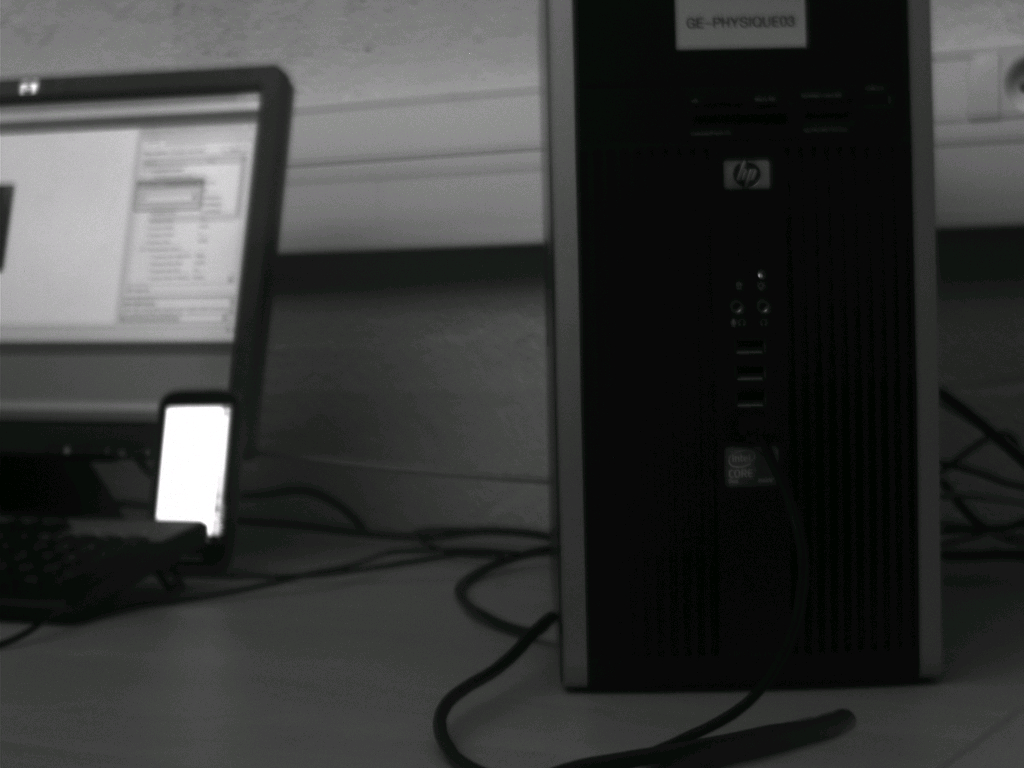
\includegraphics[width=0.3\linewidth]{Pictures/wolff/0.jpg}
	}
	\subfigure[45\textdegree]{\label{fig:oneb}
	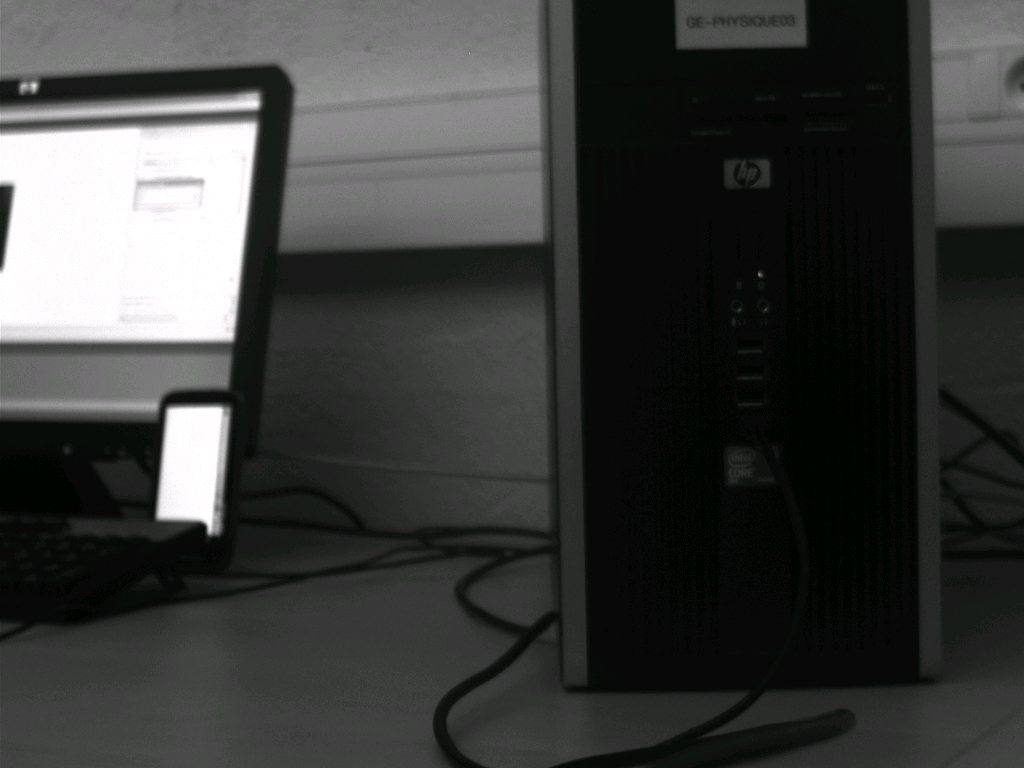
\includegraphics[width=0.3\linewidth]{Pictures/wolff/45.jpg}
	}
	\subfigure[90\textdegree]{\label{fig:onethree}
	
\includegraphics[width=0.3\linewidth]{Pictures/wolff/90.jpg}
	}
	\caption{Pictures in different angles of polarizer}
	\label{fig:one}
\end{figure}

\subsection{Wolff's method}
Before taking any pictures, we set the autoexposure and gain of the camera to be manual because we want to keep everything of camera the same, so that we can eliminate any effect from camera itself.\\
\\
After taking pictures with the polarizer orientation: 0\textdegree, 45\textdegree, 90\textdegree, we first compute the total light intensity $I$ based on the equation:
$$
I = I_{0} + I_{90}
$$

\subsection{Least Mean Square method}

\section{Step Measurement}


\section{Conclusion}

\section{References}

{[}1{]} -http://www.measurecentral.com

\end{document}